%!TEX root = ../../../thesis.tex

% Introduction
Water metering is becoming increasingly common throughout the world~\cite{Chang2012}.
Sourcing and processing drinkable water is an expensive task.
Cheap and reliable methods for reading water meters is important.
As supplies of drinkable water become constrained, volumetric pricing will become increasingly common.
Harvesting energy at the location of metering would eliminate the need for batteries.
If energy harvesting could be done without moving parts, lower component wear should lead to increased service life versus mechanical meters.
This chapter investigates the feasibility of using streaming cell technology as a means of powering electronic water meters.

\Cref{chap:part1_streamingCellHarvesters} discussed electric power generation from streaming cells.
A \SI{0.2}{\micro\percent} conversion efficiency from water flow and pressure was demonstrated.
Also, streaming voltage was found to be directly proportional to the pressure across a cell.
Can that pressure dependence be used as a method to meter water consumption while generating power? Probably.
However, questions like this are only relevant if the harvester is feasible.
Its feasibility is dictated by whether or not it can provide enough energy.
To find that out, the following questions must be answered:
\begin{enumerate}
  \item What quantity of energy is there available to harvest?
  \item What fraction can be harnessed?
  \item How much power do we need?
\end{enumerate}
The second question was answered in \cref{chap:part1_streamingCellHarvesters}, (\SI{0.0002}{\percent}); and the third will be answered in \cref{chap:part1_energyHarvestingRequirements}.
This chapter estimates the quantity of energy available for harvesting in a typical domestic setting.

% Edit checkpoint 2015-09-16 19:14


\section{Trends in Water Metering}

  %
  In New Zealand - Auckland City, Tauranga City, Nelson City, Whangarei District, and the Tasman District have already implemented water metering~\cite{WaterNewZealand2011}.
  For residents of Wellington, New Zealand's capitol city, water metering is optional.
  In metered locations, meter readers must manually read the display of each meter; a long and laborious task.

  % Automatic meter reading systems
  Automatic meter reading systems (AMR) are an alternative method of collecting that data.
  Hamilton City Council is trialling such systems in remote areas in the hopes of adopting them for wide-spread use.
  There are two types of automatic meter reading systems:
  an external reader (with communication interface) that attaches to a compatible meter, or an all-in-one unit that meters and reports usage.
  These systems offer advantages separate from taking away the laborious job of meter reading.
  Increased billing frequency helps customers reduce their consumption by giving more frequent feedback.
  They remove the need to access the customer's property~\cite{Chang2012}.
  Electronic analysis of the meters readings provides an easy way to detect water leaks.

  % Leakages
  It is estimated that \SI{10}{\percent} of post-meter water consumption is due to leakage in the residential sector~\cite{Britton2013}.
  Measuring night-time water flow is a convenient way of estimating flow due to leakage.
  Britton et al.\ show that communicating with customers whose homes showed signs of leakage that a night-time flow reduction of \SI{89}{\percent} is achievable.
  In contrast, a control group's night-time usage increased by over \SI{50}{\percent} during the same time-frame.
  The benefits of automatic water metering are not limited to billing, but improving the network as a whole.

  % Installation
  \begin{figure}
    \centering
    \includegraphics[width=0.9\textwidth]{content/pt1/02-WirelessWaterMeter/graphics/meter}
    \caption{\label{fig:Photo_DomesticWaterMeter}Photo showing a domestic water meter, and installation, (Kent PSMT 25mm) typical of an Auckland residential area.}
  \end{figure}
  Domestic water meters are typically installed at a property's boundary in a plastic box set into the ground.
  An installation typical for an Auckland residential area is shown in \cref{fig:Photo_DomesticWaterMeter}.
  The meter is installed over five meters into the property from the road-side.
  It is not feasible to connect it to a source of power because of its location.
  No commercially available domestic energy harvesting water meters, suitable for burial, exist on the market as of January 2015.

  % Approaches
  \begin{figure}
    \centering
    \label{fig:Photo_waterwareMeter}
    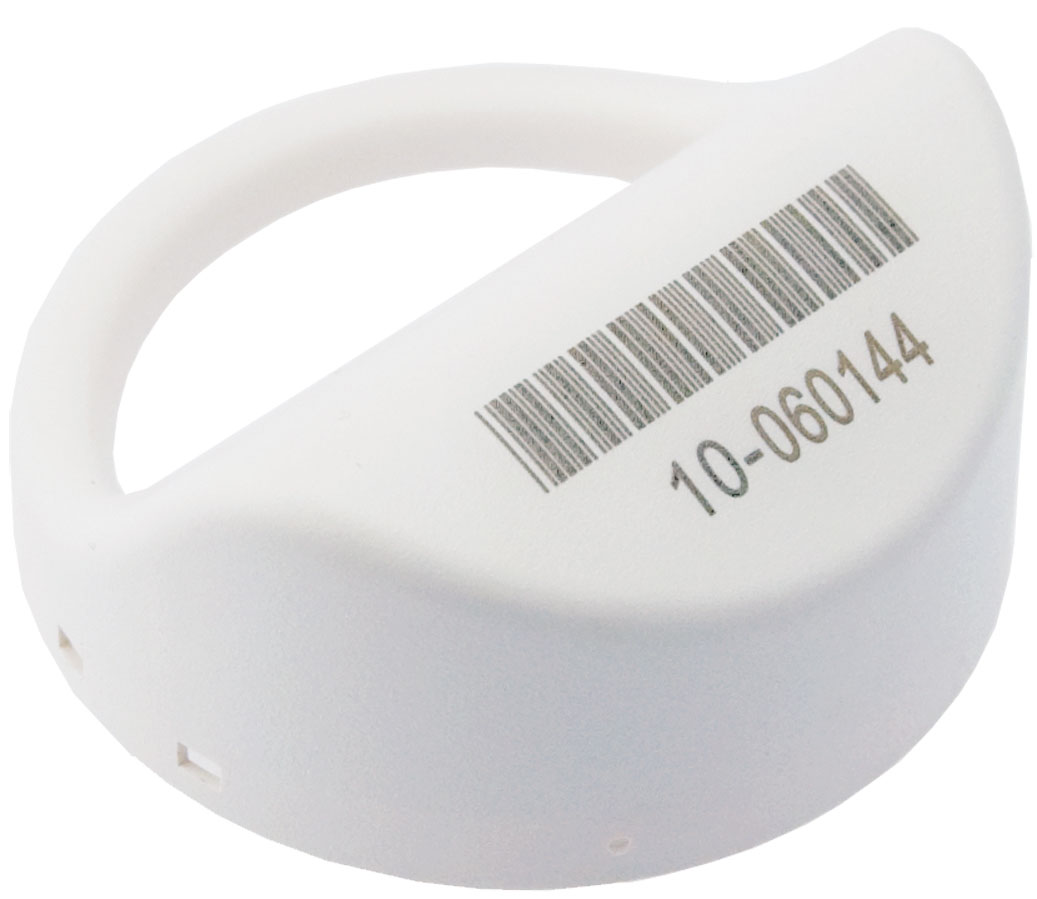
\includegraphics[width=0.5\textwidth]{content/pt1/02-WirelessWaterMeter/graphics/hydro-WMBUSWLESSM}
    \caption[Photo of a wireless transmitting module from Watercare NZ.]{
      Photo of a wireless transmitting module from Watercare NZ.
      The device attaches to a compatible water meter and contains its own battery~\cite{BMeters2014}.
    }
  \end{figure}
  A common configuration for wireless automatic meter reading is to have a reader/transmitter device that is separate to the meter itself.
  Such a device usually attaches to the meter's display or has a wire connecting it to the meter.
  Being detachable and tamper-proof means it must be powered by batteries.
  A commonly stated battery life for such units is ten years~\cite{BMeters2014}, close to a battery's shelf-life.
  We investigate the possibility of replacing these batteries with a streaming cell based energy harvester.
  A harvester removes the need for batteries, but needs to be plumbed into the water feed.
  For this reason the resulting device would most likely replace the meter, as opposed to being an attachment.


  \section{Mechanical Design of a Harvester}

    % Issues with scaling
    In \cref{chap:part1_streamingCellHarvesters}, energy was converted between fluid-mechanical to electrical using a single channel.
    Harvesting for electronic water meters will require more energy than that channel could produce.
    There are multiple ways of increasing the output power of the channel design used in \cref{chap:part1_streamingCellHarvesters}:
    the channel can be widened, doubling the width will double the output power; multiple channels can be stacked together, multiplying the output by the number of channels formed.
    Scaling the harvester is not considered a problem, but the pressure drop it develops is.
    High fluid resistance is inevitable since practical efficiencies are only obtained when the internal dimensions are small.

    % Intended harvester design
    \begin{figure}
      \centering
      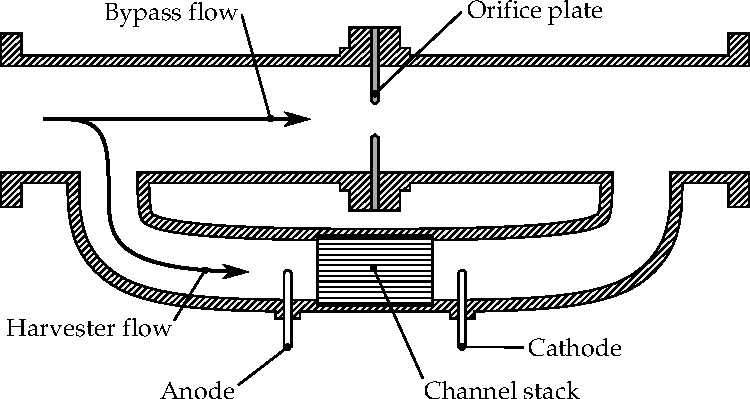
\includegraphics[width=0.9\textwidth]{content/pt1/02-WirelessWaterMeter/graphics/harvester}
      \caption{\label{fig:Diagram_harvester}Diagram showing the intended design of streaming cell harvester suitable for domestic connection.}
    \end{figure}
    To control the pressure drop across the harvester, the mechanical design shown in~\cref{fig:Diagram_harvester} is proposed.
    It gives the capability of controlling the hydrodynamic resistance of the unit as a whole by means an orifice plate.
    The plate sits in the ``main line'' causing a pressure differential in proportion to the flow rate.
    An orifice plate with a hole equal in diameter to the main pipe causes no pressure differential as it causes no flow obstruction.
    Conversely, a plate without a hole forces all liquid through the harvester, causing the maximum pressure differential.
    Using an appropriate sized orifice plate, the customer will be unaware of the harvester's presence and a suitable pressure differential will be developed.
    For the sake of analysis we assume the orifice plate will be sized to match the pressure loss of a mechanical meter.
    This assumption means the amount of harvestable energy is equal to the amount dissipated in a mechanical water meter.
    The following section quantifies the amount of energy a water meter dissipates over an average week in a typical Auckland home.


  \section{Quantifying Harvestable Energy}
  \label{sect:part1-WirelessWaterMeter-QuantifyingHarvestableEnergy}

    % Recap
    Using a bypass pipe with an orifice plate, the pressure drop across a streaming cell energy harvester can be controlled.
    The following calculations are based on the assumption that the streaming cell energy harvester will be set to collect the same amount of energy already lost inside a typical mechanical meter.

    % Water usage information
    \begin{table}
      \centering
      \begin{tabular}{r l|r|r|l}
        Item                    & Measurement & Summer & Winter & Unit\\
        \hline\hline
        \multirow{4}{*}{Shower} & Duration    & 6.6    & 7.0    & minutes\\
                                & Volume      & 50.0   & 52.5   & litres\\
                                & Flow        & 8.1    & 8.0    & litres/minute\\
                                & Frequency   & 0.9    & 0.9    & /person/day\\
        \hline
        \multirow{2}{*}{Washing}& Volume      & 122    & 123    & litres\\
                                & Frequency   & 0.35   & 0.36   & /person/day\\
        \hline
        \multirow{2}{*}{Toilet} & Volume      & 6.6    & 6.8    & litres\\
                                & Frequency   & 4.9    & 4.5    & /person/day\\
      \end{tabular}
      \caption{
          \label{tab:consumption_figures}
          Average usage characteristics for a shower, washing machine and toilet as obtained from Heinrich's water usage report~\cite{Heinrich2008}.
        }
    \end{table}
    Heinrich monitored water consumption of 51 homes throughout Auckland in 2008~\cite{Heinrich2008}.
    His report shows the majority of domestic water is consumed by the shower (\SI{30}{\percent}), washing machine (\SI{27}{\percent}) and toilet (\SI{20}{\percent}).
    Together these account for over \SI{75}{\percent} of domestic water consumption.
    Data from \cref{tab:consumption_figures} was used to build a typical water usage profile.
    Heinrich published a similar report in 2007 that contained water flow profiles, the flow profile of the toilet has been taken from that report~\cite{Heinrich2007}.

    % Profile
    \begin{figure}
      \centering
      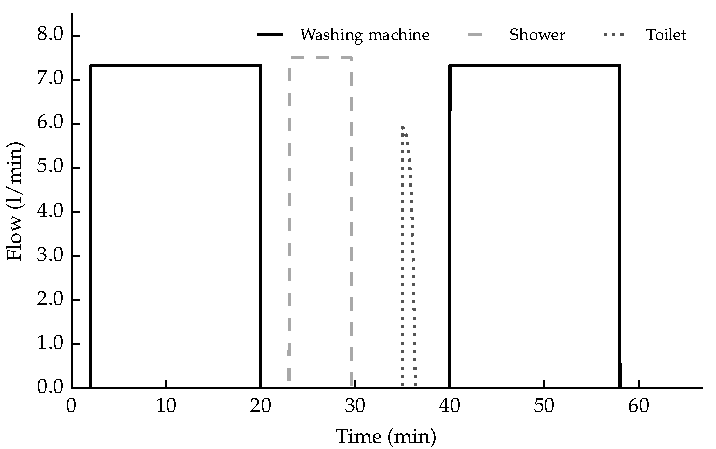
\includegraphics[width=\linewidth]{content/pt1/02-WirelessWaterMeter/graphics/graph_profile}
      \caption[Graph showing a water consumption profile of constructed instances of washing machine use, a shower and a toilet flush.]{
          Graph showing a water consumption profile of constructed instances of washing machine use, a shower and a toilet flush.
          The washing machine's wash and rinse cycles are separated in time.}
      \label{fig:profileSample}
    \end{figure}
    \Cref{fig:profileSample} shows the flow rates for each of the three items considered (toilet, shower and washing machine).
    Volumes for each of the events, and flow profile of the toilet, match the measurements reported by Heinrich.
    Specifically, the total volumes for each are: \SI{122}{\litre}, \SI{49.5}{\litre} and \SI{6.22}{\litre} for the washing machine, shower and toilet respectively.

    % Pressure loss
    \begin{figure}
        \centering
        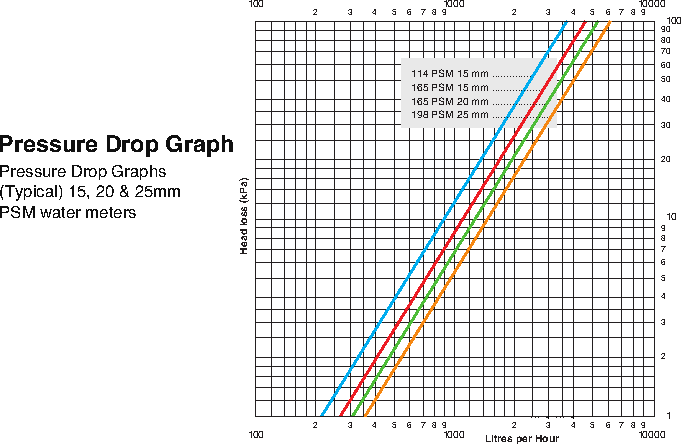
\includegraphics[width=\linewidth]{content/pt1/02-WirelessWaterMeter/graphics/Kent-PSM-HeadLoss}
        \caption{
            \label{fig:headloss}
            Log-log graph showing the pressure developed across the Kent PSM series mechanical water meters. Taken from~\cite{Elster2008}.
        }
    \end{figure}
    The Kent 25-PSMT series mechanical water meter is the most commonly installed water meter in the Auckland district~\cite{WatercareNewZealand2014}.
    \Cref{fig:headloss} shows the head-loss, or pressure differential, versus flow rate for the Kent PSM range of meters.
    The following equation was created to describe the trace representing the \SI{25}{\milli\meter} PSMT meter:
    \begin{equation}
        \Delta P = e^{3.725\thinspace log(flow) - 9.5}
        \label{eqn:Flow_to_pressure_25mmPSMT}
    \end{equation}
    \begin{figure}
        \centering
        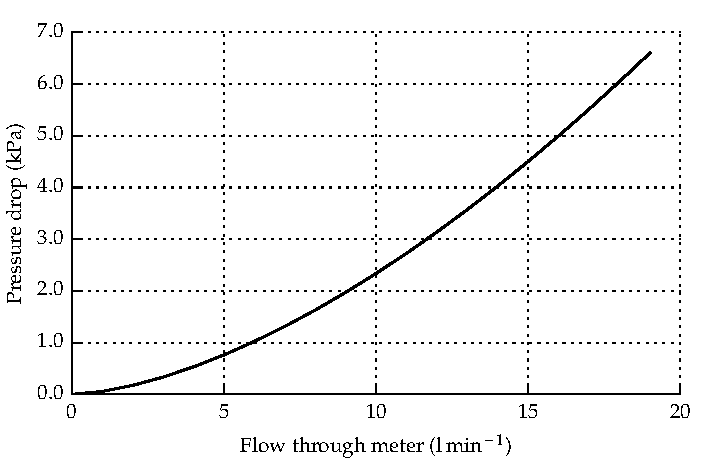
\includegraphics[width=\linewidth]{content/pt1/02-WirelessWaterMeter/graphics/graph_pressureLoss}
        \caption{Graph showing fitted curve to the pressure loss graph presented as \cref{fig:headloss}.}
        \label{fig:headloss_fit}
    \end{figure}
    \Cref{eqn:Flow_to_pressure_25mmPSMT} is plotted in \cref{fig:headloss_fit} on linear scales.

    % Calculating power loss
    Knowing the pressure differential as a function of flow provides a means of converting between flow and power dissipation.
    Like an electrical resistance, power dissipated by a fluid-flow obstruction is the product of the difference in driving force across the resistance and the flow through it.
    In this case the driving force is pressure and the flow is volumetric.
    \begin{align}
      \label{eqn:pressure_flow_to_power}
      power &= pressure \cdot flow\nonumber \\
      Watt &= Pascal \cdot \frac{cubic meter}{second}\nonumber \\
      \frac{kg\cdot m^{2}}{s^{3}} &= \frac{kg}{m\cdot  s^{2}} \thinspace \frac{m^{3}}{s}
    \end{align}
    \Cref{eqn:pressure_flow_to_power} shows the units that will be used to determine power dissipation and ensures they balance.
    \begin{figure}
        \centering
        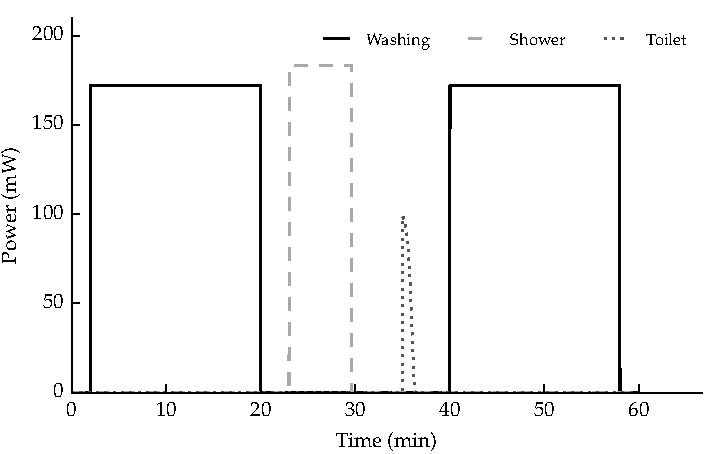
\includegraphics[width=\linewidth]{content/pt1/02-WirelessWaterMeter/graphics/graph_harvest}
        \caption{Graph of calculated power dissipation in a typical domestic mechanical water meter for each of the sample profile events.}
        \label{fig:powerDissipated_meter}
    \end{figure}
    \begin{table}
      \centering
      \begin{tabular}{r|r}
          Washing & \SI{172}{\joule}\\
          Shower  & \SI{72.6}{\joule}\\
          Toilet  & \SI{5.07}{\joule}
      \end{tabular}
      \caption{
        \label{tab:energy_dissipation_figures}
        Calculated energy dissipation within a mechanical water meter for a single washing machine cycle, shower and toilet use.
      }
    \end{table}
    Running the profiles of \cref{fig:profileSample} through \cref{eqn:Flow_to_pressure_25mmPSMT}, with relevant unit conversions, yields~\cref{fig:powerDissipated_meter}.
    It shows the power dissipated within the water during each event.
    Integrating each trace with respect to time gives the total energy lost over the course of each.
    Those energy figures are provided in~\cref{tab:energy_dissipation_figures}.

    % Total energy available
    \begin{figure}
        \centering
        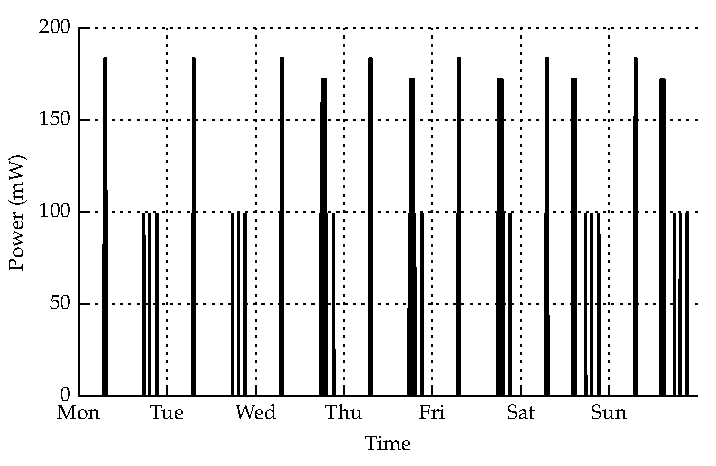
\includegraphics[width=\linewidth]{content/pt1/02-WirelessWaterMeter/graphics/graph_profileEnergy}
        \caption{
          \label{fig:profile_powerDissipation}
          Graph of power dissipation within a mechanical water meter over a week for a two occupant dwelling.
        }
    \end{figure}
    Average use frequencies for each event type are reported by Heinrech and are shown earlier in~\cref{tab:consumption_figures}.
    Using these figures, and by selecting appropriate times of day, an energy dissipation profile representative of one week was constructed.
    Five uses of a washing machine, fourteen showers, and fifty-six toilet flushes occur during this time.
    This profile is shown as~\cref{fig:profile_powerDissipation}.
    The profile fits usage figures of a home having two occupants, although most homes have more than two occupants.
    A systematic bias toward underestimating typical water usage has been used where possible.
    This underestimation also occurs by not including water use by means other than washing machines, showers or toilets.
    The intention is that the feasibility of harvesting, if the results showed near a possibility, would be more robust in light of these biases.
    \begin{table}
      \centering
      \begin{tabular}{r|r}
          Washing & \SI{860}{\joule}\\
          Shower  & \SI{1020}{\joule}\\
          Toilet  & \SI{283.9}{\joule}
      \end{tabular}
      \caption{
          \label{tab:energy_dissipation_total_figures}
          Calculated total energy dissipation over a period of one week within a mechanical water meter for typical use of a washing machine, shower and toilet.
      }
    \end{table}
    \Cref{tab:energy_dissipation_total_figures} combines the energy dissipation for each event type over a week.
    The total energy dissipated in the meter during such a week is \SI{2.16}{\kilo\joule}.
    Daily energy available is expected to fluctuate due to sporadic use of the washing machine in most homes.
    Ignoring washing machine use, indicative of weekday consumption, the quantity of harvestable energy is expected to be about \SI{280}{\joule} per day.

    % Summary
    Knowing the quantity of energy available to a harvester is a key factor determining its feasibility.
    The efficiency of converting energy into the electrical domain was measured in~\cref{chap:part1_streamingCellHarvesters} and was found to be \SI{0.2}{\micro\percent}.
    Based on that figure the measured cell would collect \SI{560}{\nano\joule} of energy per day from a two person home.
    Energy output that low is unlikely to be sufficient for automatic meter reading.
    The literature indicates the efficiency measured in~\cref{chap:part1_streamingCellHarvesters} was low.
    It may still be possible to close the gap between what we can produce and what we need.
    The amount of energy required to run an electronic water meter is estimated next.

    % Edit checkpoint 2015-09-16 19:48
